%%%%%%%%%%%%%%%%%%%%%%%%%%%%%%%%%%%%%%%%%%%%%%%%%%%%%%%%%%%%%
%   LaTeX-Arbeitsvorlage, Version 5.15                 	  	%
%   Autor: 		Mirco Lukas <http://mircol.de>              %
%   Lizenz: 	The MIT License (MIT)						%
%   Updates: 	https://github.com/MircoL/LatexTemplateDE   %
%%%%%%%%%%%%%%%%%%%%%%%%%%%%%%%%%%%%%%%%%%%%%%%%%%%%%%%%%%%%%

\def\dokumentTyp{Skript} 		% oder
%\def\dokumentTyp{Thesis}	% oder
%\def\dokumentTyp{Mitschrift}	% oder
%\def\dokumentTyp{Buch} 			% oder
%\def\dokumentTyp{Praesentation}

\def\hauptsprache{ngerman}
%\def\andereSprachen{english}


%%%%%%%%%%%%%%%%%%%%%%%%%%%%%%%%%%%%%%%%%%%%%%%%%%%%%%%%%%%%%
%   LaTeX-Arbeitsvorlage, Version 5.15                	  	%
%   Autor: 		Mirco Lukas <http://mircol.de>              %
%   Lizenz: 	The MIT License (MIT)						%
%   Updates: 	https://github.com/MircoL/LatexTemplateDE   %
%%%%%%%%%%%%%%%%%%%%%%%%%%%%%%%%%%%%%%%%%%%%%%%%%%%%%%%%%%%%%

\RequirePackage{xstring}

\makeatletter
	\@ifundefined{dokumentTyp}{%
		\errmessage{DokumentTyp muss angegeben werden!} %
		\stop %
	}
\makeatother

\IfStrEqCase{\dokumentTyp}{
	{Skript}{\documentclass[12pt,ngerman,openany,numbers=noenddot,listof=totoc,bibliography=totoc,oneside]{scrbook}}%
	{Thesis}{\documentclass[12pt,ngerman,openany,numbers=noenddot,listof=totoc,bibliography=totoc,oneside]{scrbook}}%
	{Mitschrift}{\documentclass[a4paper,12pt,ngerman,oneside]{scrartcl}}%
	{Praesentation}{\documentclass{beamer}}%
}[\errmessage{Ungueltiger Dokumenttyp: \dokumentTyp}\stop]


% =====================================================
%    Kompatibilitätseinstellungen für ältere Versionen
% =====================================================
% V5.9+	\providecommand{\hauptsprache}{ngerman}
	\providecommand{\andereSprachen}{english,polish}

% =====================================================
%    Pakete
% =====================================================

% sollte möglichst weit oben stehen
\usepackage{morewrites}

\usepackage{array}

\usepackage[xcolor,pdftex,rightbars]{changebar}

\usepackage{graphicx}
	\usepackage{epstopdf}

\usepackage{amsmath}

\usepackage{amssymb}

\usepackage[main=\hauptsprache,\andereSprachen]{babel}

% Tabelle farbig markieren: \columncolor{wunschfarbe} \rowcolor{}, \cellcolor{}
\usepackage{colortbl}

\usepackage{enumitem}

\usepackage{environ}

\usepackage{esint}

\usepackage{eurosym}

\usepackage[OT2, T2A,TS1,T1]{fontenc}


\usepackage[utf8]{inputenc}

\usepackage{listings}

\usepackage{lipsum}

\usepackage{ifthen}

\usepackage{ifsym}

% erlaubt mehrseitige Tabellen:  \begin{longtable}{|l|r|c|p{2cm}|} \hline ... \end{longtable}
\usepackage{longtable}

\usepackage{mVersion}
\increaseBuild

\usepackage{makeidx}

\usepackage{multicol}

% Workaround for Linux with texlive

\providecommand{\oeschfamily}{\em}
\usepackage{pgfkeys}

\usepackage{polski}

% m u s s  vor hyperref stehen!o
\providecommand{\zeilenabstand}{singlespacing}
\usepackage[\zeilenabstand]{setspace}

\usepackage{soul}

\usepackage{tcolorbox}



\usepackage[\hauptsprache]{varioref}

\usepackage{wasysym}

\usepackage{xspace}

\usepackage{xargs}

\usepackage{yfonts}
% Lade Pakete abhängig vom DokumentTyp.
\IfStrEqCase{\dokumentTyp}{
	{Skript}{
		\usepackage[a4paper]{geometry}
		\usepackage[hyphens]{url}
		\usepackage[pdftex,pdfborderstyle={/S/U/W 1}]{hyperref}
	}
	{Thesis}{
		\usepackage[a4paper]{geometry}
		\usepackage[hyphens]{url}
		\usepackage[pdftex,pdfborderstyle={/S/U/W 1}]{hyperref}
	}
	{Mitschrift}{
		\usepackage{fancyhdr}
		\usepackage[a4paper]{geometry}
		\usepackage[hyphens]{url}
		\usepackage[pdftex,pdfborderstyle={/S/U/W 1}]{hyperref}
		\let\chapter\section
	}
	{Praesentation}{

		\usecolortheme{whale}

		\newcommand{\fip}[1][]{\frametitle{\insertsection\xspace##1}\pause}
		\newcommand{\finp}[1][]{\frametitle{\insertsection\xspace##1}}

		\usefonttheme{professionalfonts}

		\setbeamercovered{invisible}  % Overlays auf den Folien

		\setbeamertemplate{footline}{
			\begin{beamercolorbox}[sep=1.8em,wd=\paperwidth,leftskip=0.5cm,rightskip=0.5cm]{footlinecolor}
			\end{beamercolorbox}%
			\insertsectionnavigationhorizontal{\paperwidth}{}{\hskip0pt plus1filll}
		}

		\setbeamertemplate{footline}{
			\begin{minipage}[c]{4cm}
				\get{Version 5/all/Titel}
			\end{minipage}
			\begin{minipage}[l]{4cm}
				\ifthenelse{\equal{\get{Version 5/Praesentationen/TitelKurz}}{}}{\get{Version 5/all/Titel}}{\get{Version 5/Praesentationen/TitelKurz}}
			\end{minipage}
			\begin{minipage}[c]{2cm}
				\StrSubstitute{\get{all/Autoren}}{&}{\par}
			\end{minipage}
			\hfill
			\begin{minipage}[c]{1.2cm}
				Folie \insertframenumber\ (\inserttotalframenumber)
			\end{minipage}
		}
	}
}

% m u s s   hier stehen!
\setlength{\marginparwidth}{2cm}
\usepackage{todonotes}


% =====================================================
%    Eigene Befehle
% =====================================================
\newcommand{\andd}{\wedge}
	\newcommand{\bigandd}{\bigwedge}

\newcommand{\aufgabe}[1]{%
	\command{\aktuelleAufgabe}{#1}%
	\section*{Aufgabe \aktuelleAufgabe}%
}
	\newcommand{\teilaufgabe}[1]{\paragraph*{\underline{TA \aktuelleAufgabe.#1}}}
	\newcommand{\aktuelleAufgabe}{1}

\newboolean{isAppendixSet}
	\let\appendixOld\appendix
	\renewcommand{\appendix}{\ifthenelse{\boolean{isAppendixSet}}{}{\appendixOld\setboolean{isAppendixSet}{true}}}

\newcommand{\blitz}{\lightning\xspace}

\newcommand{\countAutoren}[1]{\newcounter{autorenC}\setcounter{autorenC}{#1}}

% Nicht \dh, sonst Kollision mit dem Buchstaben ð (Eth)
\newcommand{\dhe}{d.\,h.\xspace}
\newcommand{\Dhe}{D.\,h.\xspace}

\newcommand{\ellipse}{.\hspace*{-.1em}.\hspace*{-.1em}.}

\newcommand{\fallunterscheidung}[3][]{\ensuremath{#1 \left\{\begin{array}{cl}#2\\#3\end{array}\right.}}
	\newcommand{\fuer}{&\text{für }}
	\newcommand{\sonst}{&\text{sonst}}

\newcommand{\get}[1]{\pgfkeysvalueof{/VorlageVersion5/#1}}

\newcommand{\idr}{i.\,d.\,R.\xspace}
\newcommand{\Idr}{I.\,d.\,R.\xspace}

\newcommand{\length}[1]{\ensuremath{|#1|}}

\newcommand{\name}[1]{\mbox{\textsc{#1}}}

\newcommand{\neuerbegriff}[1]{\tcbox[size=small,on line,colframe=red!75!black,colback=blue!5!white,fontupper=\normalsize]{#1}\xspace}

\newcommand{\neuerbegriffIdx}[2][]{\ifthenelse{\equal{#1}{}}{\index{#2}\neuerbegriff{#2}}{\index{#1}\neuerbegriff{#2}}}

\makeindex

\newcommand{\obda}{o.\,B.\,d.\,A.\xspace}
\newcommand{\Obda}{O.\,B.\,d.\,A.\xspace}

\makeatletter
	\def\colorref@i		{\text{\textmarker{yellow}{(i)}}}
	\def\colorref@ii	{\text{\textmarker{green}{(ii)}}}
	\def\colorref@iii	{\text{\textmarker{red}{(iii)}}}
	\def\colorref@iv	{\text{\textcolor{white}{\textmarker{blue}{(iv)}}}}
\makeatother
\newcounter{colorrefCtr}
\def\colorref(#1){ %
	\setcounter{colorrefCtr}{#1} %
	\makeatletter %
		\csname colorref@\roman{colorrefCtr}\endcsname%
	\makeatother
}

\newcommand{\sio}{s.\,o.\xspace}
\newcommand{\Sio}{S.\,o.\xspace}
\newcommand{\siu}{s.\,u.\xspace}
\newcommand{\Siu}{S.\,u.\xspace}

\newcommand{\orr}{\vee}
	\newcommand{\bigorr}{\bigvee}

\newcommand{\textmarker}[2]{\sethlcolor{#1}\hl{#2}}

\newcommand{\ua}{u.\,a.\xspace}
\newcommand{\Ua}{U.\,a.\xspace}

\newcommand{\va}{v.\,a.\xspace}
\newcommand{\Va}{V.\,a.\xspace}


\newcommand{\wiki}[1]{\href{#1}{Wikipedia}}

\newcommand{\zb}{z.\,B.\xspace}
\newcommand{\Zb}{Z.\,B.\xspace}

\newcommand{\zt}{z.\,T.\xspace}
\newcommand{\Zt}{Z.\,T.\xspace}


\IfStrEqCase{\dokumentTyp}{
	{Skript}{
		\newcommand{\qed}{\hfill\ensuremath{\square}}
	}
	{Mitschrift}{
		\newcommand{\qed}{\hfill\ensuremath{\square}}
	}
	{Praesentation}{
		\newcommand{\itemz}{\item[\RIGHTarrow]}
	}%
}



% =====================================================
%    Eigene Umgebungen
% =====================================================
\newcommand{\bspT}{}
\newenvironmentx{beispiel}[2][1={}, 2={}]{%
	\renewcommand{\bspT}{#2}
	\paragraph{Beispiel\xspace#1}%
		\begin{quotation}%
			\setlength{\parindent}{0em}\noindent%
			\ifthenelse{\equal{\bspT}{o} \OR \equal{\bspT}{b}}{\vspace*{-2em}}{}%
}{%
	\ifthenelse{\equal{\bspT}{u} \OR \equal{\bspT}{b}}{\vspace*{-1em}}{}%
	\end{quotation}%
}

\newenvironmentx{beispiele}[2][1={}, 2={}]{%
	\renewcommand{\bspT}{#2}
	\paragraph{Beispiele\xspace#1}%
	\begin{quotation}%
		\setlength{\parindent}{0em}\noindent%
		\ifthenelse{\equal{\bspT}{o} \OR \equal{\bspT}{b}}{\vspace*{-2em}}{}%
	}{%
	\ifthenelse{\equal{\bspT}{u} \OR \equal{\bspT}{b}}{\vspace*{-1em}}{}%
	\end{quotation}%
}

\newenvironmentx{beweis}[2][1={}, 2={}]{%
	\renewcommand{\bspT}{#2}
	\paragraph{Beweis\xspace#1}%
	\begin{quotation}%
		\setlength{\parindent}{0em}\noindent%
		\ifthenelse{\equal{\bspT}{o} \OR \equal{\bspT}{b}}{\vspace*{-1em}}{}
	}{%
	\ifthenelse{\equal{\bspT}{u} \OR \equal{\bspT}{b}}{\vspace*{-1.3em}}{}%
	\qed%
	\ifthenelse{\equal{\bspT}{u} \OR \equal{\bspT}{b}}{\vspace*{.5em}}{}%
	\end{quotation}%
}

\newenvironment{enumeratealpha}{\begin{enumerate}[label={\alph*)}]}{\end{enumerate}}

\newenvironment{enumerateAlpha}{\begin{enumerate}[label={\Alph*)}]}{\end{enumerate}}

\newenvironment{enumerateroman}{\begin{enumerate}[label={\roman*)}]}{\end{enumerate}}

\newenvironment{enumerateRoman}{\begin{enumerate}[label={\Roman*)}]}{\end{enumerate}}


\newcommand{\tmpQx}{}
\newcommand{\kHand}[1]{%
	\IfStrEqCase{#1}{%
		{e}{e\hspace*{-.5em}\raisebox{.05em}{\reflectbox{\c{}}}\hspace*{-.2em}}%
		{a}{a\hspace*{-.6em}\raisebox{.05em}{\reflectbox{\c{}}}\hspace*{-.1em}}%
	}[\errmessage{Ogonek nur unter 'a' und 'e'!}\stop]
}
\newcommand{\kFraktur}[1]{%
	\IfStrEqCase{#1}{%
		{e}{e\hspace*{-.1em}\raisebox{.05em}{\reflectbox{\c{}}}\hspace*{-.2em}}%
		{a}{a\hspace*{-.15em}\raisebox{.05em}{\reflectbox{\c{}}}\hspace*{-.15em}}%
	}[\errmessage{Ogonek nur unter 'a' und 'e'!}\stop]
}
\newenvironmentx{quotex}[2][1={},2={}]{%
	\renewcommand{\tmpQx}{#1}
	\begin{quote}%
		\IfStrEqCase{#2}{
			{tt}{ \texttt{#1} }%
			{hand}{ \let\k\kHand \oeschfamily }%
			{fraktur}{  \let\k\kFraktur \frakfamily }%
		}[ \normalfont ]
}{%
		\ifthenelse{\equal{\tmpQx}{}}{}{\par \mbox{} \hfill \normalfont --- \emph{\tmpQx}}%
	\end{quote}%
}
\newenvironmentx{quotationx}[2][1={},2={default}]{%
	\renewcommand{\tmpQx}{#1}
	\begin{quotation}%
		\IfStrEqCase{#2}{
			{tt}{ \texttt{#1} }%
			{hand}{ \oeschfamily }%
			{fraktur}{ \frakfamily }%
			{default}{ \normalfont }%
		}[ \errmessage{Ungueltiger Parameter: \#2 muss 'tt' oder 'hand' oder 'fraktur' sein!}\stop ]
}{%
		\ifthenelse{\equal{\tmpQx}{}}{}{\par \mbox{} \hfill \normalfont --- \emph{\tmpQx}}%
	\end{quotation}%
}


% =====================================================
%    Farbige Boxen (tcolorbox) und Indizes
% =====================================================
\tcbuselibrary{listings,breakable}

\newcommand{\boxnummer}{\thetcbcounter}
\newtcolorbox[auto counter,number format=\arabic,list inside=blueboxes]{blueboxIdx}[2][box\boxnummer]{%
	colframe=blue!75!black,fonttitle=\bfseries,title={#2},phantomlabel={#1},breakable%
}

\newtcolorbox[use counter from=blueboxIdx,number format=\arabic,list inside=yellowboxes]{yellowboxIdx}[2][box\boxnummer]{%
	colframe=yellow!99,fonttitle=\bfseries,title={\textcolor{black}{#2}},phantomlabel={#1},breakable%
}

\newtcolorbox[use counter from=blueboxIdx,number format=\arabic,list inside=greenboxes]{greenboxIdx}[2][box\boxnummer]{%
	colframe=green,fonttitle=\bfseries,title={\textcolor{black}{#2}},phantomlabel={#1},breakable%
}

\newtcolorbox[number format=\arabic]{redbox}[1][]{%
	colframe=red!99,fonttitle=\bfseries,title={\textcolor{black}{Achtung!}},phantomlabel={#1},breakable%
}



% =====================================================
%    Listings einrichten
% =====================================================

\lstset{literate=
	{á}{{\'a}}1 {é}{{\'e}}1 {í}{{\'i}}1 {ó}{{\'o}}1 {ú}{{\'u}}1
	{Á}{{\'A}}1 {É}{{\'E}}1 {Í}{{\'I}}1 {Ó}{{\'O}}1 {Ú}{{\'U}}1
	{à}{{\`a}}1 {è}{{\`e}}1 {ì}{{\`i}}1 {ò}{{\`o}}1 {ù}{{\`u}}1
	{À}{{\`A}}1 {È}{{\'E}}1 {Ì}{{\`I}}1 {Ò}{{\`O}}1 {Ù}{{\`U}}1
	{ä}{{\"a}}1 {ë}{{\"e}}1 {ï}{{\"i}}1 {ö}{{\"o}}1 {ü}{{\"u}}1
	{Ä}{{\"A}}1 {Ë}{{\"E}}1 {Ï}{{\"I}}1 {Ö}{{\"O}}1 {Ü}{{\"U}}1
	{â}{{\^a}}1 {ê}{{\^e}}1 {î}{{\^i}}1 {ô}{{\^o}}1 {û}{{\^u}}1
	{Â}{{\^A}}1 {Ê}{{\^E}}1 {Î}{{\^I}}1 {Ô}{{\^O}}1 {Û}{{\^U}}1
	{œ}{{\oe}}1 {Œ}{{\OE}}1 {æ}{{\ae}}1 {Æ}{{\AE}}1 {ß}{{\ss}}1
	{ű}{{\H{u}}}1 {Ű}{{\H{U}}}1 {ő}{{\H{o}}}1 {Ő}{{\H{O}}}1
	{ç}{{\c c}}1 {Ç}{{\c C}}1 {ø}{{\o}}1 {å}{{\r a}}1 {Å}{{\r A}}1
	{€}{{\EUR}}1 {£}{{\pounds}}1 {~}{{\textasciitilde}}1
}

\definecolor{myGray}{RGB}{220,225,225}

\lstset{
	backgroundcolor=\color{myGray},
	numbers=left,
	breakautoindent=true,
	tabsize=4,
	frame=single,
	breaklines=true,
	postbreak=\raisebox{0ex}[0ex][0ex]{\ensuremath{\color{red}\hookrightarrow\space}},
	caption=\texttt\lstname
}

\definecolor{javared}{rgb}{0.6,0,0} % for strings
\definecolor{javagreen}{rgb}{0.25,0.5,0.35} % comments
\definecolor{javapurple}{rgb}{0.5,0,0.35} % keywords
\definecolor{javadocblue}{rgb}{0.25,0.35,0.75} % javadoc
\definecolor{javablue}{RGB}{0,37,189} % javadoc

\lstset{language=Java,
	basicstyle=\ttfamily,
	keywordstyle=\color{javapurple}\bfseries,
	stringstyle=\color{javablue},
	commentstyle=\color{javagreen},
	morecomment=[s][\color{javadocblue}]{/**}{*/},
	numbers=left,
	numberstyle=\tiny\color{black},
	numbersep=10pt,
	tabsize=4,
	showspaces=false,
	showstringspaces=false
}

% =====================================================
%    Programmierdokumentation
% =====================================================
\definecolor{eclipsemodifier}{RGB}{143,0,83}
\definecolor{eclipsevar}{RGB}{0,37,189}
\newcommand{\documentationxMargin}{15pt}
\newenvironment{documentationx}{
	\fboxsep1mm
	\newcommand{\Parameter}[2][]{%
		\ifthenelse%
			{\equal{##1}{}}%
			{}%
			{%
				\IfStrEqCase{##1}{%
					{boolean}{\textcolor{eclipsemodifier}{##1}}%
					{bool}{\textcolor{eclipsemodifier}{##1}}%
					{byte}{\textcolor{eclipsemodifier}{##1}}%
					{char}{\textcolor{eclipsemodifier}{##1}}%
					{double}{\textcolor{eclipsemodifier}{##1}}%
					{short}{\textcolor{eclipsemodifier}{##1}}%
					{int}{\textcolor{eclipsemodifier}{##1}}%
					{float}{\textcolor{eclipsemodifier}{##1}}%
				}[##1]%
				\ %
			}%
		\textcolor{eclipsevar}{##2}%
	}

	\newcommand{\Pkgdef}[2]{%
		\pgfqkeys{/documentationx/pkg/##1}{
			name/.initial = {},
			description/.initial = {},
		}%
		\pgfqkeys{/documentationx/pkg/##1}{##2}%
		\noindent%
		\fbox{\textcolor{eclipsemodifier}{\texttt{package}} \texttt{\pgfkeysvalueof{/documentationx/pkg/##1/name}}}:
		\begin{addmargin}[\documentationxMargin]{0pt}
			\pgfkeysvalueof{/documentationx/pkg/##1/description}
		\end{addmargin}
	}
	\newcommand{\Classdef}[2]{%
		\pgfqkeys{/documentationx/class/##1}{
			name/.initial = {},
			description/.initial = {},
			modifier/.initial = {},
			type/.initial = {}
		}%
		\pgfqkeys{/documentationx/class/##1}{##2}%
		\noindent%
		\begingroup
			\texttt{
				\ifthenelse%
					{\equal{}{\pgfkeysvalueof{/documentationx/class/##1/modifier}}{}}%
					{}%
					{\textcolor{eclipsemodifier}{\pgfkeysvalueof{/documentationx/class/##1/modifier}}\ }%
				\ifthenelse%
					{\equal{}{\pgfkeysvalueof{/documentationx/class/##1/type}}{}}%
					{}%
					{\textcolor{eclipsemodifier}{\pgfkeysvalueof{/documentationx/class/##1/type}}\ }%
				\pgfkeysvalueof{/documentationx/class/##1/name}%
			}%
	%	\ifthenelse%
	%		{\equal{\pgfkeysvalueof{/documentationx/class/##1/description}}{}}%
	%		{}%
	%		{%
				\normalfont :
				\begin{addmargin}[\documentationxMargin]{0pt}
					\pgfkeysvalueof{/documentationx/class/##1/description}
				\end{addmargin}
	%		}%
		\endgroup%
	}
	\newcommand{\Vardef}[2]{%
		\pgfqkeys{/documentationx/var/##1}{
			name/.initial = {},
			description/.initial = {},
			modifier/.initial = {},
			type/.initial = {}
		}%
		\pgfqkeys{/documentationx/var/##1}{##2}%
		\noindent%
		\begingroup
			\texttt{%
				\ifthenelse%
					{\equal{}{\pgfkeysvalueof{/documentationx/var/##1/modifier}}{}}%
					{}%
					{\textcolor{eclipsemodifier}{\pgfkeysvalueof{/documentationx/var/##1/modifier}}\ }%
				\ifthenelse%
					{\equal{}{\pgfkeysvalueof{/documentationx/var/##1/type}}{}}%
					{}%
					{\textcolor{eclipsemodifier}{\pgfkeysvalueof{/documentationx/var/##1/type}}\ }%
				\textcolor{eclipsevar}{\pgfkeysvalueof{/documentationx/var/##1/name}}%
				\ifthenelse%
					{\equal{\pgfkeysvalueof{/documentationx/var/##1/description}}{}}%
					{}%
					{%
						\normalfont :
						\begin{addmargin}[\documentationxMargin]{0pt}
							\pgfkeysvalueof{/documentationx/var/##1/description}
						\end{addmargin}
					}%
			}%
		\endgroup%
	}
	\newcommand{\Methoddef}[2]{%
		\pgfqkeys{/documentationx/method/##1}{
			name/.initial = {},
			description/.initial = {},
			modifier/.initial = {},
			type/.initial = {} % return type
		}
		\pgfqkeys{/documentationx/method/##1}{##2}%
		\noindent%
		\begingroup
			\texttt{
				\ifthenelse%
					{\equal{}{\pgfkeysvalueof{/documentationx/method/##1/modifier}}{}}%
					{}%
					{\textcolor{eclipsemodifier}{\pgfkeysvalueof{/documentationx/method/##1/modifier}}\ }%
				\ifthenelse%
					{\equal{}{\pgfkeysvalueof{/documentationx/method/##1/type}}{}}%
					{}%
					{\textcolor{eclipsemodifier}{\pgfkeysvalueof{/documentationx/method/##1/type}}\ }%
				\pgfkeysvalueof{/documentationx/method/##1/name}%
				\ifthenelse%
					{\equal{\pgfkeysvalueof{/documentationx/method/##1/description}}{}}%
					{}%
					{%
						\normalfont :
						\begin{addmargin}[\documentationxMargin]{0pt}
							\pgfkeysvalueof{/documentationx/method/##1/description}
						\end{addmargin}
					}%
			}%
		\endgroup%
	}
}

% =====================================================
%    Initiale Konfiguration
% =====================================================

\clubpenalty = 10000

\widowpenalty = 10000

\displaywidowpenalty = 10000

\makeatletter
	\@removefromreset{footnote}{chapter}
\makeatother

% Paragraphenüberschriften immer mit einem Punkt beenden. Kann durch die Stern-Variante "\paragraph*{title}" unterdrückt werden.
\renewcommand\paragraphmark[1]{.}

\let\epsilonOld\epsilon
\let\epsilon\varepsilon

\let\phiOld\phi
\let\phi\varphi


% =====================================================
%    Deklaration der Variablen
% =====================================================

\pgfqkeys{/VorlageVersion5}{
	all/Autoren/.initial					= {},
	all/Titel/.initial	 					= {},
	all/Untertitel/.initial 				= {},
	all/VersionPraefix/.initial 			= {},
	all/Version/.initial 					= {true},
	all/Icon/Breite/.initial				= {},
	all/Icon/URL/.initial					= {},
	all/Index/Boxen/blau/titel/.initial 	= {Liste der Sätze und Definitionen},
	all/Index/Boxen/blau/zeigen/.initial 	= {false},
	all/Index/Boxen/gelb/titel/.initial 	= {Liste der Beispiele},
	all/Index/Boxen/gelb/zeigen/.initial 	= {false},
	all/Index/Boxen/gruen/titel/.initial 	= {Liste der Fragen},
	all/Index/Boxen/gruen/zeigen/.initial 	= {false},
	all/Index/Begriffe/titel/.initial 		= {Index},
	all/Index/Begriffe/zeigen/.initial 		= {false},
	all/Index/Literatur/titel/.initial 		= {Literaturverzeichnis},
	all/Index/Literatur/zeigen/.initial 	= {false},
	Skript/AnmerkungenTitelseite/.initial 	= {},
	Mitschriften/Vorlesungsname/.initial 	= {},
	Mitschriften/Typ/.initial 				= {},
	Mitschriften/LfdNr/.initial 			= {},
	Mitschriften/Gruppe/.initial 			= {},
	Mitschriften/Headerhoehe/.initial		= {42pt},
	Buecher/Widmung/.initial				= {},
	Buecher/Modus/.initial					= {rl},
	Praesentationen/TitelKurz/.initial		= {},
	Praesentationen/Institut/lang/.initial	= {},
	Praesentationen/Institut/kurz/.initial	= {},
	Thesis/AkademischerGrad/kurz/.initial	= {},
	Thesis/AkademischerGrad/lang/.initial	= {},
	Thesis/Fach/Nominativ/.initial			= {},
	Thesis/Fach/Genitiv/.initial			= {},
	Thesis/UniName/lang/.initial			= {},
	Thesis/UniName/kurz/.initial			= {},
	Thesis/EingereichtBei/.initial			= {},
	Thesis/BetreuungDurch/.initial			= {},
	Thesis/Abgabedatum/.initial				= {},
	Thesis/Versicherung/zeigen/.initial		= {true},
	Thesis/Versicherung/text/.initial		= {},
	Thesis/Versicherung/ort/.initial		= {}
}


% =====================================================
%    Generiere passende Titelseiten, Kopfzeilen etc.
% =====================================================
\AtBeginDocument{
	% Zulässige Werte testen
	\begingroup
		\newcommand{\checkbool}[1]{\ifthenelse{\equal{\get{#1}}{true} \OR \equal{\get{#1}}{false}}{}{\errmessage{Boolean '#1' muss 'true' oder 'false' sein!}\stop}}
		\checkbool{all/Version}
		\checkbool{all/Index/Boxen/blau/zeigen}
		\checkbool{all/Index/Boxen/gelb/zeigen}
		\checkbool{all/Index/Boxen/gruen/zeigen}
		\checkbool{all/Index/Begriffe/zeigen}
		\checkbool{all/Index/Literatur/zeigen}
		\checkbool{Thesis/Versicherung/zeigen}
		% ------------------------------------------------------------------------
	\endgroup

	\setVersion{\get{all/VersionPraefix}}
	\IfStrEqCase{\dokumentTyp}{
		{Skript}{%
			\thispagestyle{empty}
			\vspace*{4em}
			\begin{center}
				\ifthenelse{\equal{\get{all/Titel}}{}}{}{{\Huge \textbf{\get{all/Titel}}\par}}
				\ifthenelse{\equal{\get{all/Untertitel}}{}}{}{\vspace*{.5em}{\large\textbf{\get{all/Untertitel}}\par}}
			\end{center}
			\begin{flushright}
				\ifthenelse{\equal{\get{Skript/AnmerkungenTitelseite}}{}}{}{{\em \vspace*{1em}\get{Skript/AnmerkungenTitelseite}\par}}
				\ifthenelse{\equal{\get{all/Version}}{true}}{Version: \version, }{}\today\par\vspace*{1em}
				\StrSubstitute{\get{all/Autoren}}{&}{\par}
			\end{flushright}
			\begin{center}
				\IfFileExists{titel.png}{%
					
\includegraphics[width=\get{all/Icon/Breite}\textwidth]{titel.png}\par%
					\ifthenelse{\equal{\get{all/Icon/URL}}{}}{}{{\tiny \href{\get{all/Icon/URL}}{Quelle}}}
				}{}
			\end{center}
			\newpage

			\pagenumbering{Roman}
			\newpage
			\tableofcontents

			\newpage

			\newpage
			\pagenumbering{arabic}
		}
		{Thesis}{%
			\ifthenelse{\equal{\get{all/Autoren}}{}}{\errmessage{Kein Autor bei der Thesis angegeben!}\stop}{}
			\ifthenelse{\equal{\get{all/Titel}}{}}{\errmessage{Kein Titel bei der Thesis angegeben!}\stop}{}

			% an anderer Stelle führt dies zu einem Stacküberlauf ("Tex capacity exceeded, sorry...")!
			% \newcommand\eingereichtBei{}
			% \StrSubstitute{\get{Thesis/EingereichtBei}}{&}{,\par}[\eingereichtBei]
			% \newcommand\betreuungDurch{}
			% \StrSubstitute{\get{Thesis/BetreuungDurch}}{&}{,\par}[\betreuungDurch]

			\thispagestyle{empty}
			\vspace*{4em}
			\begin{center}
				%\ifthenelse{\equal{\get{Thesis/AkademischerGrad/kurz}}{}}{}{%
					%\get{Thesis/AkademischerGrad/kurz}arbeit zur Erlangung des akademischen Grades\par	eines \get{Thesis/AkademischerGrad/lang} \get{Thesis/Fach/Genitiv}%
					%Abschlussarbeit im Fach \get{Thesis/Fach/Nominativ}%
				%}
				%\\
				\ifthenelse{\equal{\get{Thesis/UniName/lang}}{}}{}{\textbf{\get{Thesis/UniName/lang}}\par}
				\IfFileExists{titel.jpg}{%
					\vspace*{1em}%
					
\includegraphics[width=\get{all/Icon/Breite}\textwidth]{titel.jpg}\par%
					\ifthenelse{\equal{\get{all/Icon/URL}}{}}{}{{\tiny \href{\get{all/Icon/URL}}{Quelle}}}
				}{}
				\ifthenelse{\equal{\get{all/Titel}}{}}{}{{\Huge \textbf{\get{all/Titel}}\par}}
				\ifthenelse{\equal{\get{all/Untertitel}}{}}{}{\vspace*{.5em}{\large\textbf{\get{all/Untertitel}}\par}}
				\vspace*{.5em}
				{\textbf{\Large \get{all/Autoren}}}
			\end{center}

			\begin{tabular}{ll}%
				\ifthenelse{\equal{\eingereichtBei}{}}{}{\noindent Eingereicht bei: & \multicolumn{1}{p{11cm}}{\eingereichtBei} \\}%
				\ifthenelse{\equal{\betreuungDurch}{}}{}{\noindent Betreuung durch: & \multicolumn{1}{p{11cm}}{\betreuungDurch} \\}%
				\noindent Abgabedatum:	 & \get{Thesis/Abgabedatum}%
			\end{tabular}
			\begin{flushright}
				\ifthenelse{\equal{\get{Skript/AnmerkungenTitelseite}}{}}{}{{\em \vspace*{1em}\get{Skript/AnmerkungenTitelseite}\par}}
				\ifthenelse{\equal{\get{all/Version}}{true}}{Version: \version}{}
			\end{flushright}

			\newpage

			\pagenumbering{Roman}
			\newpage
			\tableofcontents

			\newpage

			\newpage
			\pagenumbering{arabic}
		}
		{Mitschrift}{
			\setlength{\parindent}{0cm}
			\setlength{\headheight}{\get{Mitschriften/Headerhoehe}}
			\pagestyle{fancy}
			\newcommand{\autorTemp}{\StrSubstitute{\get{all/Autoren}}{&}{\par}}
			\expandafter\lhead{\autorTemp}
			\chead{%
				\IfFileExists{titel.jpg}{
\includegraphics[width=\get{all/Icon/Breite}\textwidth]{titel.jpg}\\}{}
				\ifthenelse{\equal{\get{Mitschriften/Gruppe}}{}}{}{Gruppe \get{Mitschriften/Gruppe}}
			}
			\rhead{\textbf{\emph{\get{Mitschriften/Vorlesungsname}}}\\\textbf{\get{Mitschriften/Typ}\ \get{Mitschriften/LfdNr}}\ifthenelse{\equal{\get{all/Version}}{true}}{\\Stand: \today}{}}
			\lfoot{}
			\cfoot{-- \thepage\ --}
			\rfoot{}

			\global\long\def\headrulewidth{0.4pt}
			\global\long\def\footrulewidth{0.4pt}
			\ifthenelse{\equal{\get{all/Titel}}{}}%
				{\section*{\get{Mitschriften/Typ}\ \get{Mitschriften/LfdNr}}}%
				{\section*{\get{all/Titel}}}

			\ifthenelse{\equal{\get{all/Untertitel}}{}}{}{\subsubsection*{\get{all/Untertitel}}}
		}
		{Praesentation}{
			\title{\get{all/Titel}}
			\subtitle{\get{all/Untertitel}}
			\StrSubstitute{\get{all/Autoren}}{&}{\par}[\autorTemp]
			\author{\autorTemp}
			\IfFileExists{titel.jpg}{\logo{titel.jpg}}{}
			\ifthenelse{\equal{\get{Praesentationen/Institut}}{}}{}{\institute{\get{Praesentationen/Institut}}}

			\frame{\titlepage}

			\frame{
				\finp
				\tableofcontents
			}
		}
	}
}

\AtEndDocument{
	\appendix


		\renewcommand{\bibname}{\get{all/Index/Literatur/titel}}
		\bibliographystyle{alphadin}
		\nocite{*}
		\bibliography{quellen}


	\IfStrEqCase{\dokumentTyp}{
		{Skript}{%
			\ifthenelse{\equal{\get{all/Index/Boxen/blau/zeigen}}{true}}{\tcblistof[\chapter]{blueboxes}{\get{all/Index/Boxen/blau/titel}}}{}

			\ifthenelse{\equal{\get{all/Index/Boxen/gelb/zeigen}}{true}}{\tcblistof[\chapter]{yellowboxes}{\get{all/Index/Boxen/gelb/titel}}}{}

			\ifthenelse{\equal{\get{all/Index/Boxen/gruen/zeigen}}{true}}{\tcblistof[\chapter]{greenboxes}{\get{all/Index/Boxen/gruen/titel}}}{}

			\newpage
			\ifthenelse{\equal{\get{all/Index/Begriffe/zeigen}}{true}}{
				\renewcommand{\indexname}{\get{all/Index/Begriffe/titel}}
				\phantomsection
				\addcontentsline{toc}{chapter}{\indexname}
				\printindex
			}{}
		}
		{Thesis}{%
			\ifthenelse{\equal{\get{Thesis/Versicherung/zeigen}}{true}}{%
				\chapter{Eigenständigkeitserklärung}%
				\ifthenelse{\equal{\get{Thesis/Versicherung/text}}{}}%
					{Ich erkläre hiermit, dass ich die vorliegende Arbeit selbständig verfasst, keine anderen als die angegebenen Quellen und Hilfsmittel benutzt sowie die diesen Quellen und Hilfsmitteln wörtlich oder sinngemäß entnommenen Ausführungen als solche kenntlich gemacht habe. \par
					\noindent Die Arbeit habe ich bisher oder gleichzeitig keiner anderen Prüfungsbehörde vorgelegt.
					\\ \\
				}{\get{Thesis/Versicherung/text}}%
				\noindent \get{Thesis/Versicherung/ort}, \get{Thesis/Abgabedatum}
				\\ \\ \\

				\noindent ......................................................

				\noindent \StrSubstitute{\get{all/Autoren}}{&}{\par}

				\newpage%
			}{}

			\ifthenelse{\equal{\get{all/Index/Boxen/blau/zeigen}}{true}}{\tcblistof[\chapter]{blueboxes}{\get{all/Index/Boxen/blau/titel}}}{}

			\ifthenelse{\equal{\get{all/Index/Boxen/gelb/zeigen}}{true}}{\tcblistof[\chapter]{yellowboxes}{\get{all/Index/Boxen/gelb/titel}}}{}

			\ifthenelse{\equal{\get{all/Index/Boxen/gruen/zeigen}}{true}}{\tcblistof[\chapter]{greenboxes}{\get{all/Index/Boxen/gruen/titel}}}{}

			\ifthenelse{\equal{\get{all/Index/Begriffe/zeigen}}{true}}{
				\renewcommand{\indexname}{\get{all/Index/Begriffe/titel}}
				\addcontentsline{toc}{chapter}{\indexname}
				\printindex
			}{}
		}
		{Mitschrift}{%
			\ifthenelse{\equal{\get{all/Index/Boxen/blau/zeigen}}{true}}{\tcblistof[\chapter]{blueboxes}{\get{all/Index/Boxen/blau/titel}}}{}

			\ifthenelse{\equal{\get{all/Index/Boxen/gelb/zeigen}}{true}}{\tcblistof[\chapter]{yellowboxes}{\get{all/Index/Boxen/gelb/titel}}}{}

			\ifthenelse{\equal{\get{all/Index/Boxen/gruen/zeigen}}{true}}{\tcblistof[\chapter]{greenboxes}{\get{all/Index/Boxen/gruen/titel}}}{}

			\ifthenelse{\equal{\get{all/Index/Begriffe/zeigen}}{true}}{
				\renewcommand{\indexname}{\get{all/Index/Begriffe/titel}}
				\addcontentsline{toc}{chapter}{\indexname}
				\printindex
			}{}
		}
		{Praesentation}{%
			\ifthenelse{\equal{\get{all/Index/Begriffe/zeigen}}{true}}{
				\newenvironment{theindex}{\let\item\par}{}

				\newcommand\indexspace{}

				\begin{frame}
					\frametitle{\get{all/Index/Begriffe/titel}}
					\printindex
				\end{frame}
			}{}
		}
	}
}



% ===========================================================================

% Die voreingestellten Werte werden verwendet, wenn sie hier nicht explizit überschrieben werden.
% Alle überflüssigen Zeilen können gelöscht werden.
\pgfqkeys{/VorlageVersion5}{
	all/Autoren						= {Tom Mohr},
	all/Titel	 					= {Softwareprojekt},
	all/Untertitel 					= {Informatiksysteme, Klasse 13},
	all/VersionPraefix 				= {1.0.0},
	all/Version 					= {true},
	all/Icon/Breite					= {.7},
	all/Icon/URL					= {},
	all/Index/Boxen/blau/titel 		= {Liste der Sätze und Definitionen},
	all/Index/Boxen/blau/zeigen 	= {false},
	all/Index/Boxen/gelb/titel 		= {Liste der Beispiele},
	all/Index/Boxen/gelb/zeigen 	= {false},
	all/Index/Boxen/gruen/titel 	= {Liste der Fragen},
	all/Index/Boxen/gruen/zeigen 	= {false},
	all/Index/Begriffe/titel 		= {Index},
	all/Index/Begriffe/zeigen 		= {true},
	all/Index/Literatur/titel 		= {Literaturverzeichnis},
	all/Index/Literatur/zeigen 		= {true}, 
%
	% Zusätzlich für Skripte
	Skript/AnmerkungenTitelseite 	= {},
%
	% Zusätzlich für Mitschriften
	Mitschriften/Vorlesungsname 	= {},
	Mitschriften/Typ 				= {\"Ubung},
	Mitschriften/LfdNr 				= {},
	Mitschriften/Gruppe 			= {},
	Mitschriften/Headerhoehe		= {42pt},
%
	% Zusätzlich für Bücher
	Buecher/Widmung					= {},
	Buecher/Modus					= {rl},
%
	% Zusätzlich für Präsentationen
	Praesentationen/TitelKurz		= {},
	Praesentationen/Institut/lang	= {},
	Praesentationen/Institut/kurz	= {},
%
	% Zusätzlich für Abschlussarbeiten
	Thesis/AkademischerGrad/kurz	= {},
	Thesis/AkademischerGrad/lang	= {},
	Thesis/Fach/Nominativ			= {},
	Thesis/Fach/Genitiv				= {},
	Thesis/UniName/lang				= {},
	Thesis/UniName/kurz				= {},
	Thesis/EingereichtBei			= {},
	Thesis/BetreuungDurch			= {},
	Thesis/Abgabedatum				= {},
	Thesis/Versicherung/zeigen		= {false},
	Thesis/Versicherung/ort			= {},
	Thesis/Versicherung/text		= {}
}

% ===========================================================================
%      Hier eigene Packages einbinden und eigene Befehle definieren

\usepackage{caption}
\captionsetup{font=small,labelfont=bf}
\usepackage{graphicx}
\usepackage{rotating}
% ===========================================================================


\begin{document}

\chapter{Anforderungsdefinition}	
%\addcontentsline{toc}{chapter}{Zusammenfassung}
Dieses Projekt entsteht im Zusammenhang mit einer Schularbeit. Der Fokus liegt primär auf dem Lerninhalt und der Umsetzung. Die Eignung und Verwendbarkeit des Resultats ist sekundär.

\section{Projektinhalt}
Ziel ist es, für ein kleines fiktives Unternehmen, welches kleine Speisen (Fast Food und Snacks) verkauft, eine Kassenverwaltungssoftware zu implementieren, die den Verkauf analysiert und das Lager verwaltet.
Bisher wurden die Arbeiten ohne Verwaltungssystem durchgeführt und die Kassierung erfolge manuell.
Dadurch herrscht ein höherer Aufwand für Kassenbuch, Steuerberater und die Verwaltung der Liquiden Mittel.
Bei Einnahmezählungen kann nicht festgestellt werden, welche Produkte sich am besten Verkauft haben und ob es sich Einnahmen mit Ausgaben decken.

Besonderen Wert soll darauf gelegt werden, dass die Software ohne großen Einarbeitungsaufwand bedient werden kann, und durch die Verwendung einen modernen Technologiestacks in Zukunft einfach gewartet und verwendet werden kann.
Da es sich um ein Kassensystem handelt, sind die Anforderungen an Datensicherheit und -integrität besonders hoch.

\section{Erwartungshorizont}
Die bereits vorhandene Infrastruktur basiert auf Windows 10 Computern der x64-Architektur.
Daher muss die Anwendung mit mindestens Windows 10 oder neuer kompatibel sein.
Eine Netzwerkfähigkeit muss gewährleistet sein, um den Datenaustausch über das interne Netzwerk zu ermöglichen.
Im Verwaltungsbereich sollen Mitarbeiter Einnahmen und Produkte verwalten können.
Genannte Produkte sollen sinnvolle Eigenschaften wie Bezeichnung, Einzelpreis, Verfügbarkeit im Lager besitzen.
Die getätigten Transaktionen sollen als Statistik gespeichert und dargestellt werden, um dem Benutzer einen Überblick über die vergangenen Verkäufe zu geben.
Dabei soll die Darstellung der Daten vorerst nicht erfolgen.
Die Verarbeitung der Anfragen und Daten erfolgt über eine API, die Endpunkte für die benötigten Funktionen bieten, welche von Clients frei verwendet werden können.
Ein Client ist jedoch nicht Teil des Erwartungshorizonts.
Das Projekt muss im Zeitraum vom 27.12.2022 bis 13.03.2023 fertiggestellt werden.
Eine finanzielle Begrenzung gibt es nicht.

\chapter{Technologien}
Dieses Projekt verwenden gängige Technologien, welches die Entwicklung vereinfachen und die Integration mit anderen Systemen ermöglichen. Im folgenden werden die wesentlichen T. erklärt.

\section{C\#}
C\# (gesprochen „C-Sharp“) ist eine objektorientierte Programmiersprache, die im Auftrag von Microsoft entwickelt und 2000 veröffentlicht wurde.
Die Sprache ist grundsätzlich plattformunabhängig und wurde für die Softwareplattform .NET entwickelt.
Auf GitHub gehört sie zu den fünf am meisten verwendeten Programmiersprachen.\cite{ms-csharp}

Die Einsatzbereiche dieser Sprache sind nahezu Grenzenlos.
Schon seit Veröffentlichung entstanden Projekte in den Bereichen Webseiten, Entwicklerwerkzeuge und Kompilierer.
Durch diese einfach, moderne und flexible Sprache qualifiziert sie sich auch für dieses Projekt.
Der Zusammenschluss von C und C++ brachte diese Eigenschaften herbei und macht es somit selbst Java Entwicklern einfach, die Sprache zu verwenden.\cite{dev-csharp}

\section{HTTP}
HTTP steht für „Hypertext Transfer Protocol“ und ist das Kommunikationsprotokoll im World Wide Web (WWW).
Es ist für das Abrufen von statischen Inhalten, wie HTML-Dokumenten, vorgesehen und bildet somit die Grundlage für jeden Datenaustausch im Web als Client-Server-Protokoll.
In der Regel werden Anfragen an den Server über einen Browser gestellt, der ebenso die Antwort des Servers empfängt und darstellt.

Das  in den 1990er Entwickelte Protokoll ist erweiterbar und kann mittels TLS Verschlüsselt werden. Es lässt sich inder Anwendungsschicht im ISO/OSI-Referenzmodell einordnen.
HTTP ist zustandslos, da es keine Verbindung zwischen zwei Anfragen gibt, die nacheinander auf der selben Verbindung ausgeführt werden, kann aber mittels HTTP-Cookies für zustandshafte Sitzungen Verwendung finden.\cite{mdn-http}

HTTP-Antworten enthalten die Version des Protokolls, Header, den Statuscode der angibt, ob die Anfrage erfolgreich war (wie in Abbildung \vref{http-response} gezeigt), eine Status-Nachricht und den Körper der Nachricht mit dem angeforderten Inhalt.
HTTP-Header ermöglichen Client und Server den Austausch zusätzlicher Informationen, so z.B. für die Authentifizierung des Clients am Server, für das verwendete Caching (Pufferspeichern) oder gespeicherte Cookies.\cite{mdn-http-header}

\begin{figure}[ht]
	\centering
	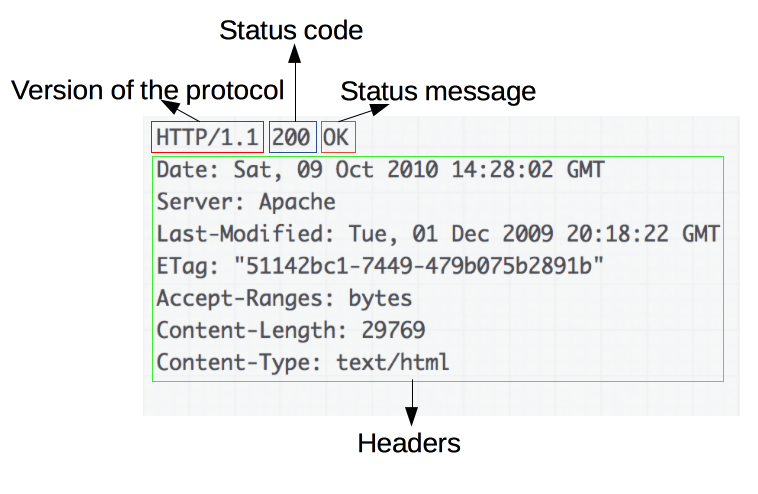
\includegraphics[width=0.7\linewidth]{http_response.png}
	\caption{Beispiel einer HTTP-Antwort}
	\label{http-response}
\end{figure}

\section{IDE}
%bearbeiten
Für eine effiziente Arbeitsweise benötige ich Programme, welche mir beim Schreiben des Quelltextes helfen und diesen für mich kompilieren, damit am Ende eine ausführbare Anwendung bereitsteht. Auch hier greife ich wieder auf eine mir bereits bekannte Lösung von Microsoft zurück: Microsoft Visual Studio 2022. Das Programm bietet hilfreiche Funktionen wie das automatische Installieren von Paketen, das farbige Markieren von Quelltexten für eine bessere Lesbarkeit und einen Kompilierer, der C-Sharp versteht. Die IDE gibt mir außerdem Möglichkeiten in meine Anwendung während der Laufzeit hereinzuschauen, um Fehler schneller finden zu können sowie die Korrektheit der Vorgänge zu überprüfen.

\section{Git}
Git ist ein ausgereiftes, aktiv gepflegtes Open-Source-Projekt, das ursprünglich 2005 von Linus Torvalds, entwickelt wurde.
Eine erstaunliche Anzahl von Softwareprojekten verlässt sich auf Git für die Versionskontrolle, einschließlich kommerzieller Projekte sowie Open Source.
Im Gegensatz anderer Versionskontrollsoftware lässt sich Git bei der Versionshistorie des Dateibaums nicht von den Namen der Dateien täuschen, stattdessen konzentriert sich Git auf den Dateiinhalt selbst.
Somit gehört es mit zu den Leistungsstärksten seiner Art.
Die Integriergerät des Quellcodes war bei der Entwicklung die höchste Priorität. Der SHA1 Algorithmus wird für die Sicherung der Verzeichnissen verwendet. So wird der Verlauf vor Änderungen beschützt.

Git zeichnet sich ebenso durch seine Flexibilität aus: es Unterstützt verschiedene Arten von Entwicklerworkflows, die nichtlinear sind. Es eignet sich somit für alle Größen von Projekten.\cite{git}
Durch die Einteilung von Git in drei Arbeitsbereiche können Änderungen flexibel angebracht werden.

Im Arbeitsverzeichnis (Working Directory) liegen alle Projektdateien zur Bearbeitung oder Benutzung.
Änderungen an diesen Dateien werden im Entwicklungsbereich (Staging Area) erfasst und aufbewahrt.
Um diese Änderungen zu veröffentlichen, muss ein Commit (Beitrag) erzeugt werden, welcher die Informationen der Änderungen trägt.
Diese können dann im Versionsverlauf des Git Verzeichnisses gespeichert werden. Abbildung \vref{git-sections} stellt diese Beziehungen dar.

\begin{figure}[ht]
	\centering
	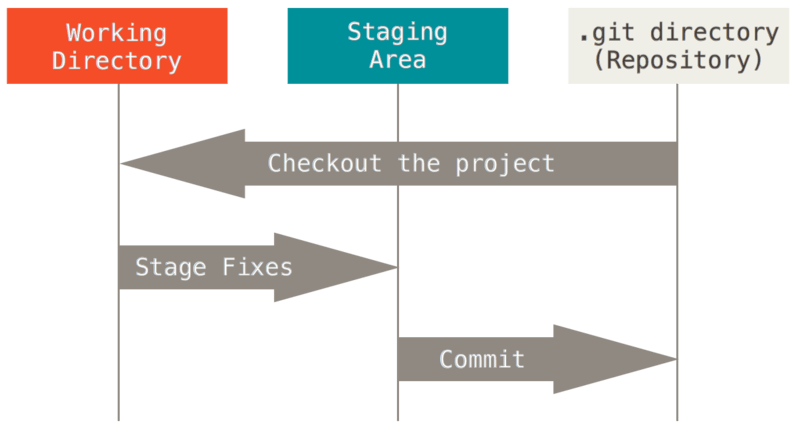
\includegraphics[width=0.8\linewidth]{git-sections.png}
	\caption{Arbeitsverzeichnis, Entwicklungsbereich, Git Verzeichnis}
	\label{git-sections}
\end{figure}

\section{SQLite}
Das relationale Datenbank-Management-System (DBMS) ist eine leichtgewichtige Lösung, die ohne Server auskommt, für eine schnelle Datenbankanbindung. Die Open-Source-Software kann in Anwendungen integriert werden, um Speicherung von Daten ohne separaten Datenbankserver zu ermöglichen. SQLite wurde in C geschrieben und ist mit vielen Betriebssystem wie Windows, Linux, MacOS, Android und iOS. Unterstützt werden grundlegende SQL-Operationen wie INSERT, UPDATE; SELECT und DELETE. Abfragen mit Aggregatfunktionen, Unterabfragen und Joins sind ebenso möglich. Durch die ACID-Konformität ist Zuverlässigkeit und Robustheit gewährleistet. Der Funtkionsumfang ist gegenüber MySQL sehr eingeschränkt. Diese Einschränkung haben jedoch keinen negativen Einfluss auf das Projekt.

\section{Kanban}
Kandban ist ein Arbeitsmodus, indem ein Projekt in kleine Arbeitspakete zerlegt wird und diese mithilfe eines Boards geplant werden können.
Das Board besteht aus Spalten TODO, In Progress, Done als einfachste Form.
Ein Vorteil dieser Arbeitsweise ist, einen direkten überblicke über getane und geplante Arbeit zu erhalten.
Du durch einzelne Spalten könne zusätzlich priorisierte Gruppen erstellt werden.
Beim Kollaborativen Arbeiten werden die Tickets, die in Bearbeitung sind, einer Verantwortlichen Person zugewiesen.
Um den Erfolg einer Arbeit in Kanban zu messen, verwendet man zwei wesentliche Metriken: die Zykluszeit, welche die benötige Zeit für eine Aufgabe misst und den Durchsatz, der die Anzahl der abgeschlossenen Daten für eine bestimmte Zeiteinheit zurückgibt. \cite{kanban}

Eine weitere Darstellungsform des Erfolgs ist das kumulatives Flussdiagramm (CFD). Es veranschaulicht die Anzahl der Elemente (Vertikale Achse) im Laufe der Zeit (Horizontale Achse). Die Zustände der Bereiche werden mir Farben gekennzeichnet, wie Abbildung \vref{cfd} zeigt. Sind die Verläufe der Bereiche nahezu parallel, wurde der Zeitplan eingehalten.

\begin{figure}[ht]
	\centering
	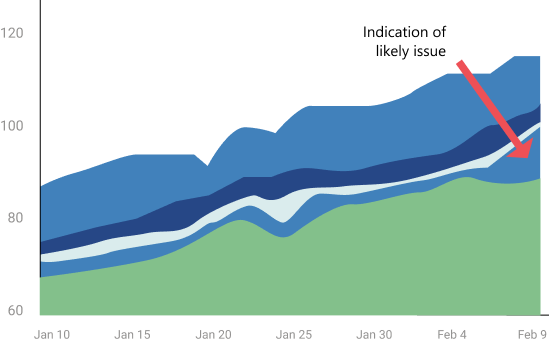
\includegraphics[width=0.7\linewidth]{kanban-cumulative-flow-2.png}
	\caption{Beispiel eines CFD mit Verschiebung im Zeitplan}
	\label{cfd}
\end{figure}

\section{Testing}
Um sicherzustellen, das die Software den gestellten Anforderungen entspricht, müssen zentrale Bestandteile dieser durch Tests abgesichert werden.
Es gibt verschiedene Arten von Test, von denen die wichtigsten Unit-Test sind.
Hierbei handelt es sich um de Prüfung isolierter Softwarebestandteile, die gegen vordefinierte Daten geprüft werden.
Zu beachten ist, das Tests keine Fehlerfreiheit garantieren können, jedoch insbesondere die Software gegen Fehler durch Erweiterungen robust machen.\cite{ms-testing}

Andere Arten von Softwaretest sind Integration- und Smoke-Test, welche als Blackboxtest zusammengefasst werden können.
Integrationstests überprüfen die einzelnen Module einer Software auf ihre Zusammenarbeit mit anderen.
So können z.B. Datenbankanbindungen und Microservices auf ihre Funktionalität geprüft werden.\cite{atlassian-testing}

Allgemein sollen Tests Sicherheit, Produktqualität und Kostenersparnisse sichern.
Wenn ein defekt in der Software nicht Zeitnah erkannt wird, steigt der Suchaufwand nach des Auslösers in komplexen Projekten enorm.
Werden Fehler in der frühen Entwicklungsphase behoben, werden so die Kosten für die weiteren Entwicklung niedriger gehalten.
Sicherheitslücken die noch vor der Veröffentlichung einer Version geschlossen werden, bieten Angreifern keine Möglichkeit eine Software zu missbrauchen.
Nebenbei sei auch erwähnt, dass eine fehlerfreie Software mehr Kundenzufriedenheit bedeutet.\cite{stm-testing}

\chapter{Authentifizierung}
Dieser Abschnitt erklärt die Arbeitsweise der implementierten Authentifizierung.

\section{HTTP-Authentifizierung}
Die Authentifizierung für HTTP soll sicherstellen, das die Anfragen eines Benutzers nur bearbeitet werden, wenn dieser dazu berechtigt ist. 
Durch die Feststellung der Identität wird die Sicherheit des Systemen gewährleistet. 
Es gibt mehrere Authentifizierungsverfahren. 
Die einfachste ist, dass der Client Benutzername und Passwort an den Server schickt, welcher diese anschließend validiert.

\paragraph{Basic Authentication}

Als am einfachsten zu Implementieren gilt das Senden und Überprüfen von Benutzername und Passwort im Klartext. 
Dies ist jedoch nur mit der Verwendung von HTTPS zu empfehlen, da die Sicherheit sonst nicht gewährleistet werden kann.

\paragraph{Digest Authentication}

Anders als bei der Basic Authentication wird das Passwort hier nicht im Klartext übertragen. 
Ein Hash des Passworts erhöht hier die Sicherheit und gibt somit nicht das Geheimnis preis.

\paragraph{Token-Based Authentication}

Statt eines Passworts kommt hier ein eindeutiges Token zum Einsatz, welches bei jeder Aufforderung mitgesendet wird. 
Der Server validiert dieses jedes mal, um die Berechtigung des Benutzers zu prüfen.
Ein Vorteil ist, dass hierbei Berechtigungen mit dem Token verknüpft sein können.

\paragraph{OAuth2 Authentication}

Dieser Standard überträgt Authentifizierungs- und Autorisierungsinformationen zwischen zwei Teilnehmern eines Netzwerks in Form eines Token.
Diese Methode soll einen einfachen Informationsaustausch für Anmeldungen ermöglichen, ohne das eine aktive Verbindung aufrechterhalten werden muss.
Der hier verwendete Token kann von dem eigenen oder sogar einem Drittanbieter bereitgestellt werden, der sein eigenes Rechtesystem verwaltet. 
Dieser teilt einem anderen Server bei einer Anfrage mit, ob der Benutzer berechtigt ist, auf diese Ressourcen zuzugreifen.
Dieses Verfahren hat den Vorteil, dass dass Passwort nur dem Server, der das Token ausstellt, bekannt sein muss, nicht jedoch dem anfragenden Server.
Diese Eigenschaften machen JWT portabel und skalierbar. 
Die Übertragung ist plattformübergreifend möglich und das Format ist kompakt. 
Der Server muss hier keine Sitzungsinformationen speichern, da ein JWT alle Informationen über die Berechtigungen enthält. 
Eine Manipulation kann sehr einfach erkannt werden, da es bei Veränderungen des Inhalts zu Fehlern bei einer Validierung der Signatur kommt.\cite{ionos-jwt}

JWTs wirken bei Single-Sign-On (SSO) unterstützend, da der Benutzer nach einer Authentifizierung einen JWT erhält, welchen er für die Anmeldung bei Anfragen an einen Server verwenden kann.

\section{JSON-Web-Token}
Eine mögliche Implementierung eines OAuth2 Token kann über JWT realisiert werden (bei der Erweiterung OpenIdConnect ist das immer der Fall).
Das JSON-Web-Token (JWT) setzt sich aus drei Teilen zusammen: 
\begin{itemize}
	\item dem \textbf{Header} mit Token-Typ und der Signaturmethode (base64-encoded),
	\item der \textbf{Payload}, welcher Informationen über den Benutzer (z.\,B. die E-Mail-Adresse) beinhaltet (base64-encoded) und 
	\item der \textbf{Signatur}, welche die Richtigkeit des Tokens bezeugen soll.\cite{jwt}
\end{itemize}

\noindent Ein Beispiel-Token mit decodiertem (Klartext-)Inhalt kann der Abbildung \vref{jwt-decoder} entnommen werden.

\begin{figure}[ht]
	\centering
	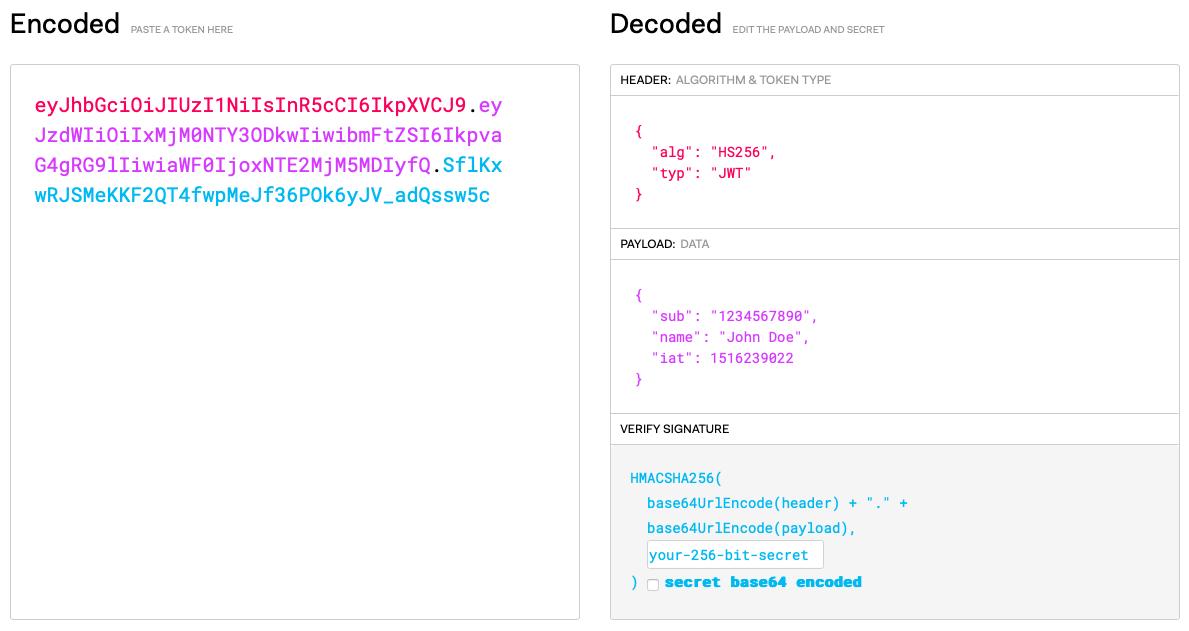
\includegraphics[width=.85\linewidth]{jwt.png}
	\caption{Vergleich von enkodiertem und dekodiertem JWT}
	\label{jwt-decoder}
\end{figure}

Dieser Standard überträgt Authentifizierungs- und Autorisierungsinformationen zwischen zwei Teilnehmern eines Netzwerks in Form einer Zeichenkette, dem Token. Diese Methode soll einen einfachen Informationsaustausch für Anmeldungen ermöglichen, ohne das eine aktive Verbindung aufrechterhalten werden muss.

Diese Eigenschaften machen JWT portabel und skalierbar. Die Übertragung ist Plattformübergreifend möglich und das Format ist kompakt. Der Server muss hier keine Sitzungsinformationen speichern, da JWT alle Informationen über die Berechtigungen enthält. Eine Manipulation ist nicht möglich, da es sonst zu Fehlern bei einer Validierung der Signatur kommt.\cite{ionos-jwt}

JWTs wirken bei Single-Sign-On (SSO) unterstützend, da der Benutzer nach einer Authentifizierung einen JWT erhält, welchen er für die Anmeldung bei Anfragen an einen Server verwenden kann.

\chapter{Backend}\label{backend}
\section{REST-API}
In diesem Projekt werden API-Endpunkte (gekapselt in sog. \emph{Controllern}) und andere Funktionen wie z.\,B. Datenbankoperationen voneinander getrennt.
Das verwendete HTTP-Framework bindet den HTTP-Request an eine Funktion, wodurch eine einfache und saubere Implementierung ermöglicht wird.
Somit können Endpunkte einfach verschoben und Integration Tests einfacher durchgeführt werden.
Annotationen mit den HTTP-Verben definieren dabei die Art der Anfrage.
Das ermöglicht, die Zugehörigkeit direkt im Quelltext abzulesen.

Die in der URL übertragenen Parameter werden direkt die der Funktion zugeordnet.
Dadurch wird sichergestellt, das die Daten aus dem Body der Anfrage dem Datentyp entsprechen, den die Funktion verarbeiten kann.
Sollte dies nicht der Fall sein, beantwortet das Framework, welches in Abschnitt \ref{backend} genauer erklärt wird, die Anfrage mit einem HTTP-Fehlercode.

Funktion geben immer ein \texttt{IActionResult} zurück, welches die Klasse \linebreak\texttt{ObjectResult} enthält.
Die hier am Wichtigsten enthaltenen Eigenschaften sind der Statuscode und der Body.
Das Framework kann somit eine HTTP-Antwort zurückgeben und gleichzeitig können Integration Tests intern, d.\,h. ohne HTTP, durchgeführt werden.
\linebreak
\linebreak
Eine Übersicht aller verfügbaren Controller ist in den Tabellen \vref{controller1} und \vref{controller2} zu finden. Zu beachten ist, dass alle Endpunkte zusätzlich zu den angegeben Statuscodes auch die Codes \texttt{401 Unauthorized} oder \texttt{403 Forbidden} bei fehlender Authentifizierung und \texttt{500 Internal Server Error} bei einer Systemfehlkonfiguration zurückgeben können.
\linebreak
\linebreak
Der nicht erwähnte Endpunkt \texttt{/Authentication/register-admin} wird benötigt, um ein Administratorkonto anzulegen.
Daher wird er nur zur Einrichtung des Systems benötigt um MUSS aus Sicherheitsgründen anschließend durch eine Firewall, \texttt{.htaccess}-Datei o.ä. blockiert werden.
Methode, Rollen, Parameter, Rückgabe und Statuscodes sind identisch mit \texttt{/Authentication/register}.

Werden Benutzerkonten von einem Administrator zentral verwaltet, sollte der Endpunkt zur Registrierung ebenso abgesichert werden.

\begin{sidewaystable}
	\caption{Controller Definitionen 1/2}
	\centering
	\label{controller1}
\begin{tabular}{llllllll}
	Controller   & Name          & Methode & Rolle     & URL       & Parameter          & Rückgabe                          & Statuscodes   \\
	Product      & GetProducts   & GET     & Seller    & /all      & null               & List\textless{}uint\textgreater{} & 200, 404      \\
	Product      & GetProduct    & GET     & Seller    & /\{id\}   & uint id            & Product                           & 200, 404      \\
	Product      & AddProduct    & POST    & Manager   & /add      & Product p          & Product                           & 201, 409      \\
	Product      & ModifyProduct & PUT     & Manager   & /\{id\}   & uint id, Product p & Product                           & 200, 404, 423 \\
	Product      & DeleteProduct & DELETE  & Manager   & /\{id\}   & uint id            & null                              & 200, 404, 423 \\
	&               &         &           &           &                    &                                   &               \\
	Price        & GetPrices     & GET     & Admin     & /all      & null               & List\textless{}Guid\textgreater{} & 200, 404      \\
	Price        & GetPrice      & GET     & Manager   & /\{id\}   & Guid id            & Price                             & 200, 404      \\
	Price        & AddPrice      & POST    & Manager   & /add      & Price p            & Price                             & 201, 409      \\
	Price        & ModifyPrice   & PUT     & Manager   & /\{id\}   & Guid id, Price p   & Price                             & 200, 404, 423 \\
	Price        & DeletePrice   & DELETE  & Manager   & /\{id\}   & Guid id            & null                              & 200, 404, 423 \\
	&               &         &           &           &                    &                                   &               \\
	Group        & GetGroups     & GET     & Manager   & /all      & null               & List\textless{}Guid\textgreater{} & 200, 404      \\
	Group        & GetGroup      & GET     & Manager   & /\{id\}   & Guid id            & Group                             & 200, 404      \\
	Group        & AddGroup      & POST    & Manager   & /add      & Price p            & Group                             & 201, 409      \\
	Group        & ModifyGroup   & PUT     & Manager   & /\{id\}   & Guid id, Price p   & Group                             & 200, 404, 423 \\
	Group        & DeleteGroup   & DELETE  & Manager   & /\{id\}   & Guid id            & null                              & 200, 404, 423 \\
	&               &         &           &           &                    &                                   &               \\
	Authenticate & Login         & POST    & Anonymous & /login    & LoginModel l       & string                            & 200           \\
	Authenticate & Register      & POST    & Anonymous & /register & RegisterModel r    & bool                              & 200           \\
	&               &         &           &           &                    &                                   &               \\
	Misc         & Ping          & GET     & Anonymous & /ping     & null               & "Pong"                            & 200          
\end{tabular}
\end{sidewaystable}

\begin{sidewaystable}
	\caption{Controller Definitionen 2/2}
	\centering
	\label{controller2}
\begin{tabular}{llllllll}
	Controller & Name             & Methode & Rolle   & URL             & Parameter      & Rückgabe                                & Statuscodes \\
	Purchase   & GetPurchases     & GET     & Seller  & /all            & null           & List\textless{}Guid\textgreater{}       & 200, 404    \\
	Purchase   & GetPurchase      & GET     & Seller  & /\{id\}         & uint id        & Purchase                                & 200, 404    \\
	Purchase   & SellPurchase     & POST    & Seller  & /sell           & Purchase p     & Guid                                    & 200         \\
	Purchase   & BuyPurchase      & POST    & Seller  & /buy            & Purchase p     & Guid                                    & 200         \\
	Purchase   & CancelPurchase   & POST    & Seller  & /cancel         & Purchase p     & Guid                                    & 200         \\
	Purchase   & RefundPurchase   & POST    & Seller  & /refund         & Purchase p     & Guid                                    & 200         \\
	Purchase   & DisposalPurchase & POST    & Manager & /dispose        & Purchase p     & Guid                                    & 200         \\
	&                  &         &         &                 &                &                                         &             \\
	Stats      & GetTotalStats    & GET     & Analyst & /total          & null           & List\textless{}TotalStats\textgreater{} & 200, 204    \\
	Stats      & GetYearStats     & GET     & Analyst & /year/\{i\}     & ushort i       & YearStats                               & 200, 404    \\
	Stats      & GetAllYearStats  & GET     & Analyst & /year/all       & null           & List\textless{}ushort\textgreater{}     & 200, 204    \\
	Stats      & GetMonthStats    & GET     & Analyst & /month/y/m      & ushort y, m    & MonthStats                              & 200, 404    \\
	Stats      & GetAllMonthStats & GET     & Analyst & /month/all      & null           & List\textless{}DateTime\textgreater{}   & 200, 204    \\
	Stats      & GetDayStats      & GET     & Analyst & /day/y/m/d      & ushort y, m, d & DayStats                                & 200, 404    \\
	Stats      & GetAllDayStats   & GET     & Analyst & /day/all        & null           & List\textless{}DateTime\textgreater{}   & 200, 204    \\
	Stats      & GetProductStats  & GET     & Analyst & /product/\{id\} & uint id        & ProductStats                            & 200, 404   
\end{tabular}
\end{sidewaystable}

\newpage
\section{Weitere Bestandteile}
Die API basiert hauptsächlich auf dem Framework \texttt{Microsoft.Entity\-Framework\-Core}.
Ein Objekt vom Typ \texttt{IHost} (Host) mit einer \texttt{IConfiguration} (Konfiguration) schafft die Grundlage der API.
Welche API-Controller eingebunden sind, die Anbindung der Datenbank sowie die Definition der Zugriffsrechte sind Informationen, die in der Konfiguration enthalten sind.

Das bereits im Framework eingebaute Werkzeug \emph{SwaggerUI} kann verwendet werden, um den Aufbau der API grafisch darzustellen und Anfragen direkt über den Browser stellen zu können.
Hier werden auch Definitionen, Kommentare und Datentypen beschrieben und wie sie in der API verwendet werden können.

\subsection{Datenbank}
Das verwendete Datenbanksystem ist SQLite.
Benutzer und Anwendungsdaten werden in zwei getrennten .db-Dateien gespeichert.
Der Grund für diese Trennung liegt in der Funktionsweise der Anbindung.
Während für die Datenbank mit den Anwendungsdaten ein Klasse vom Typ \texttt{DbContext} verwendet wird, benötigt die Verarbeitung der Benutzer und Rollen einen \texttt{IdentityDbContext}.

Damit es hier nicht zu Migrationsproblemen kommt und die Benutzerdaten bei einer Änderung der Datenstruktur nicht erneut generiert werden müssen, wurden die beiden Kontext-Klassen nicht zusammengelegt.
Außerdem macht diese Methode es möglich, Anwendungsdaten und Benutzerdaten an getrennten Orten aufzubewahren, was im Sinne der Datensicherheit und des Datenschutzes ist.

Die Klassen für Benutzer- und Rollendaten werden von den beiden Frameworks \texttt{Microsoft.\-AspNetCore\-.Identity} und \texttt{Microsoft.\-AspNetCore.\-Identity.\linebreak\-Entity\-Framework\-Core} bereitgestellt. 
Die Eigenschaften und Beziehungen der Anwendungsdaten können Abbildung \vref{data-erm} entnommen werden.

\subsection{Authentifizierung}
Damit Endpunkte verwendet werden können, muss sich der Benutzer dafür authentifizieren. 
Dieser Vorgang wird in Abbildung \vref{login-struct} beschrieben.
Die Endpunkte zum Registrieren und Anmelden sind Anonym erreichbar.
Im Body der Anfrage muss ein JSON-Objekt mitgegeben werden, welches entweder von der Klasse LoginModel oder RegisterModel abstammt.
Zweiteres enthält zusätzlich zu den Eigenschaften Username und Password des LoginModel eine Zeichenkette für die E-Mail Adresse des Benutzers.

Ist eine Anmeldung erfolgreich gewesen, sendet der Server eine Antwort mit einem JWT im Body.
Diesen muss der Client bei allen anderen Anfragen im Authorization-Header mitsenden, um vom Server Authentifiziert zu werden.

\begin{figure}[ht]
	\centering
	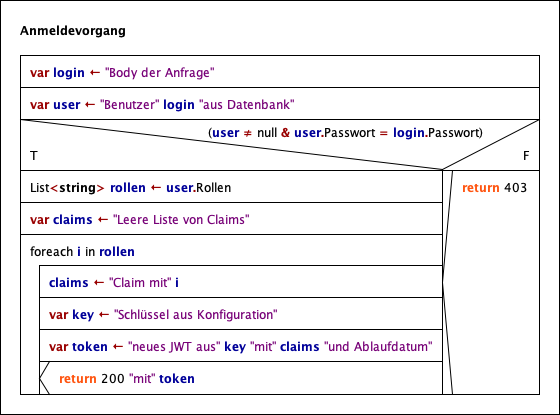
\includegraphics[width=0.7\linewidth]{Anmeldevorgang.png}
	\caption{Ablauf der Anmeldung}
	\label{login-struct}
\end{figure}

\begin{figure}[ht]
	\centering
	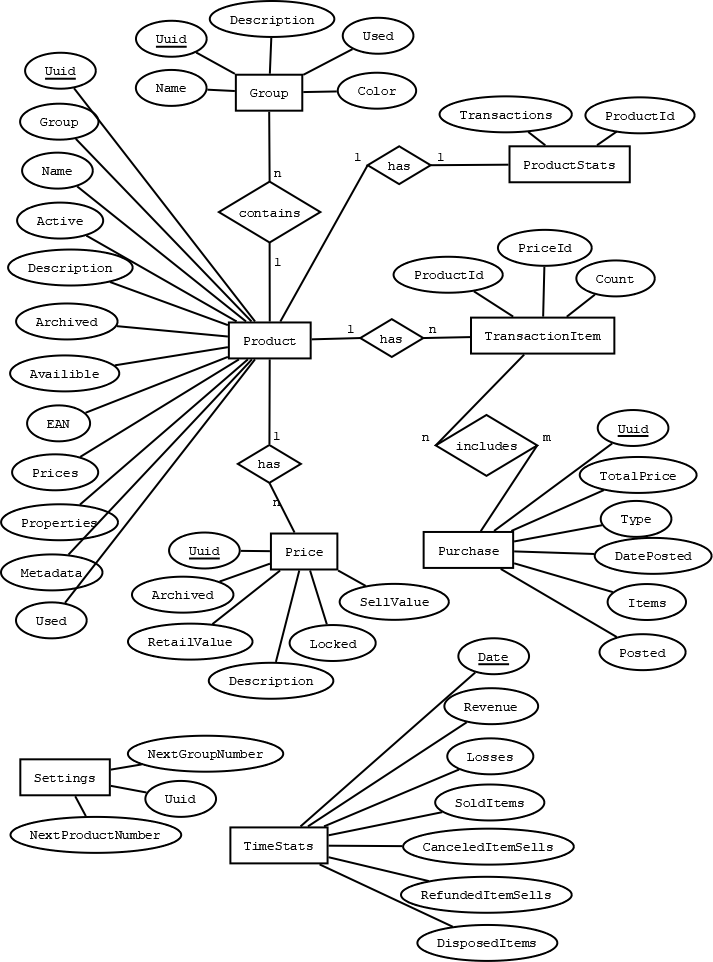
\includegraphics[width=1\linewidth]{ERM.png}
	\caption{ERM der Anwendungsdaten}
	\label{data-erm}
\end{figure}

\subsection{Verarbeitung von Anfragen}
Empfangene Anfragen werden nach einer Prüfung der Identität des Clients an den zuständigen Controller geleitet, der den angesprochenen Endpunkt enthält.
Demonstriert wird dieser Vorgang in Abbildung \vref{product-creation} anhand der Erstellung eines Produkts.

Die Kommunikation zwischen Datenbank und API findet über einen \texttt{DbContext} statt.
Dieser ermöglicht es, die verwendeten Klassen der Objekte direkt in Tabellen zu konvertieren, damit diese mit einem Befehl abgerufen und manipuliert werden können. Daher sind in der API kein vorgeschriebenen SQL-Abfragen vorhanden.

Nach Beendung der Bearbeitung der Datenbank erzeugt jeder Endpunkt ein HTTP-Fähiges Resultat, welches über den Controller an den Client zurückgegeben wird.
Eine genaue Definition der Rückgaben aller Endpunkte ist in den Tabellen \vref{controller1} und \vref{controller2} zu finden.
 
\begin{sidewaysfigure}[ht]
	\centering
	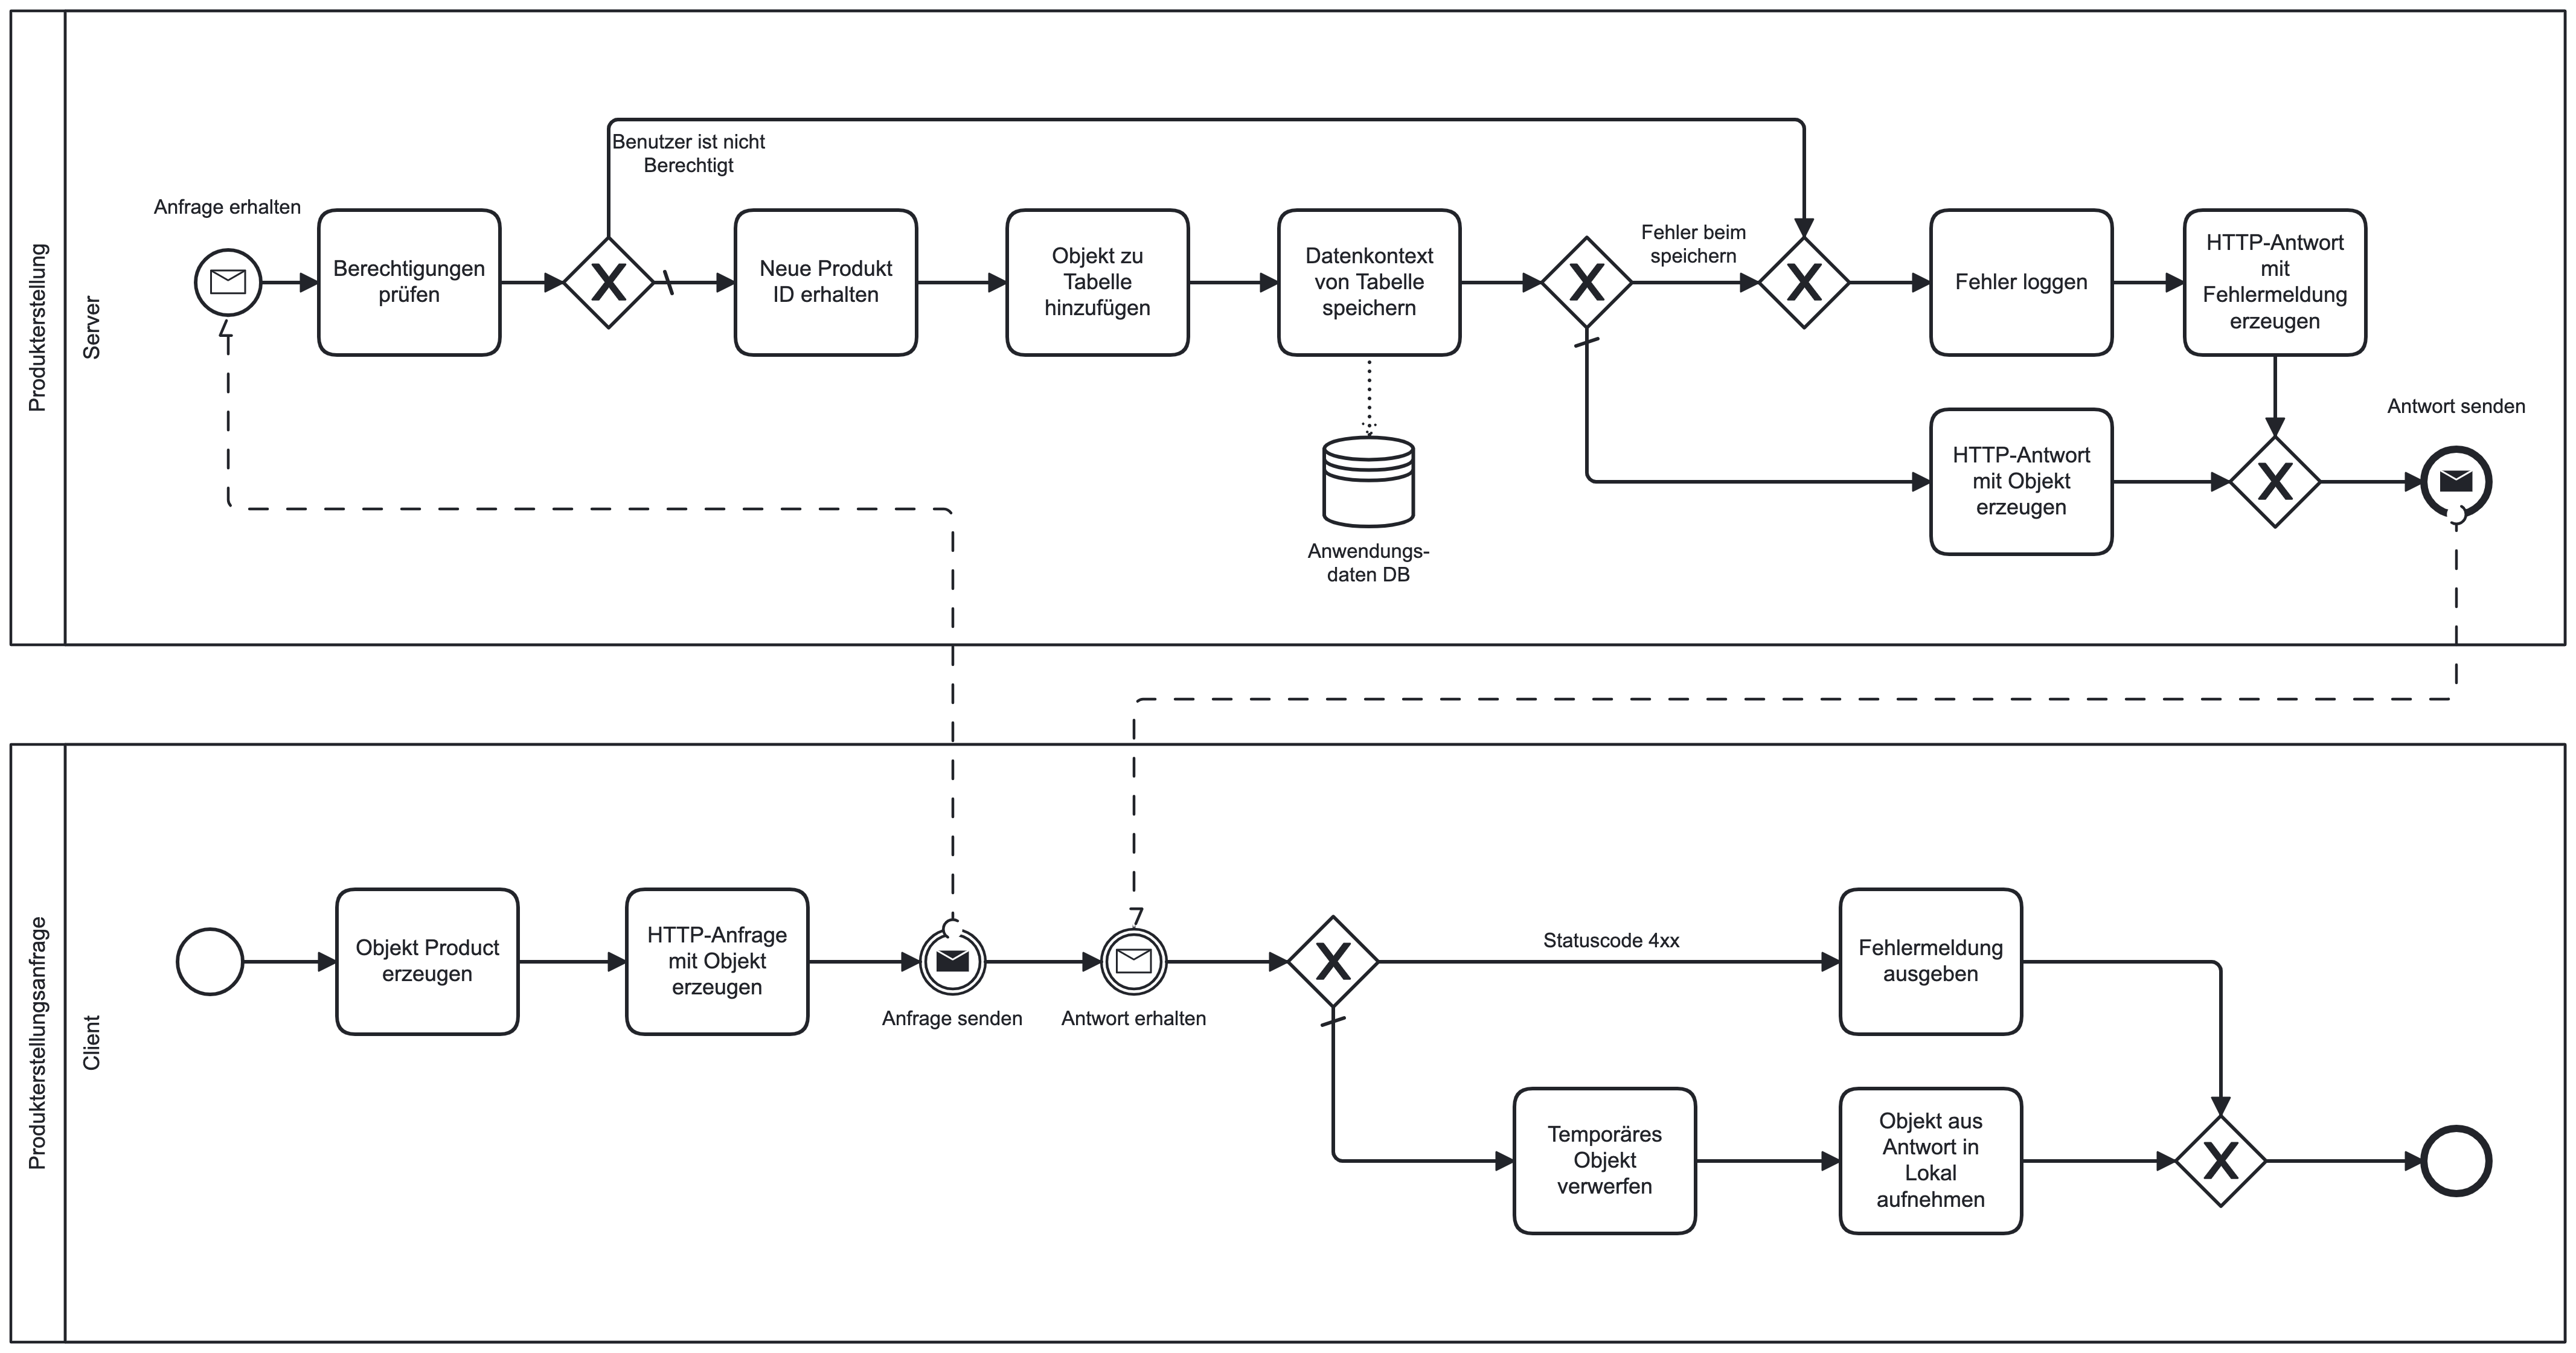
\includegraphics[width=1\linewidth]{Produkterstellung.png}
	\caption{Ablauf der Anmeldung}
	\label{product-creation}
\end{sidewaysfigure}

\chapter{Reflexion}
Die Wahl von ASP.NET Core als Framework und Mircosoft Visual C\# als Programmiersprache ist eine gute Entscheidung gewesen, da hier der geringste Einarbeitungsaufwand im Vergleich zu anderen Sprachen wie Pascal, Visual Basic oder Node.Js vorhanden war. Entscheidend ist somit die persönlich Bekannteste Sprache gewesen, woraus sich einen zeitlichen Vorteil ergab.

Während der Entwicklungsphase kamen immer wieder Probleme auf, welche die Einhaltung der zeitlichen Planung verhinderten.
Das implementieren der Authentifizierung dauerte mehr als eine geplante Woche und durch eine ungenaue Planung zu Beginn, mussten Datenmodelle in laufe der Entwicklung immer wieder geändert werden, um die gesetzten Anforderungen erfüllen zu können.

Bis zwei Wochen nach eigentlicher Fertigstellung der Datenmodelle mussten für Grundlegende Eigenschaften wie Primärschlüssel ein anderer Datentyp gewählt werden, um die Integrität in der Datenbank sicherstellen zu können.
Oft entstanden neue Ideen zur Umsetzung des Projekt oder es traten Fehler als Licht, die durch eine genauere Planung hätten vermieden werden können.
Die Funktionen der API sind weitreichend Kommentiert. Leider ließ es die Zeit nicht mehr zu, weitere innere Quelltextzeilen zu kommentieren.

Vor Start des Projekts sollte zusätzlich zu deiner implementierten API auch ein Client erstellt werden, der als Kommunikationsschnittstelle zwischen API und Benutzer fungieren sollte. Als jedoch laut Zeitplan die Entwicklung des Frontends starten müsste und das Backend bei weitem noch nicht fertig war, entfiel dieser Teil des Projekts, um die API in einer höheren Qualität entwickeln zu können.

Die erstellten Integration-Tests decken nur den Bereich der Erfolgreichen Antworten ab.
Die API besteht all diese Tests, allerdings ist ungewiss, ob bei einer falschen Verwendung der Endpunkte die richtigen Fehler angezeigt werden.
Prinzipiell ist die API so entwickelt, dass jeder Fehler aufgefangen werden kann, ohne das die Anwendung Einfriert oder Abstürzt.

SQLite ist, wie bereits erwähnt, sehr gut führ diesen Anwendungszweck geeignet.
Jedoch lassen sich API-Server und Datenbankserver nicht voneinander trennen.
Diese Eigenschaft ist im Umfeld der Projektanforderungen in Ordnung, verbietet aber den Aufstieg in eine professionellere Ebene.
MySQL oder SQL-Server wären mit den Frameworks ebenso kompatibel gewesen, hätten aber auch einen größeren Konfigurationsaufwand für dieses Projekt mitgebracht. Dieser Grund und die Kompatibilität von SQLite, mit den gleichen Plattformen wie der API-Server, gaben die Entscheidung auf das zu verwendete Datenbanksystem vor.

Das Projekte hatte einen sehr großen Lerneffekt.
Durch das Entwickeln eines, persönlich, neuen Anwendungstyps hat weitreichende Blicke in die Zukunft gebracht, um für die nächsten Projekte mehr Möglichkeiten zur Umsetzung einer Problemlösung zu haben.
Das schreiben der Dokumentation in LaTeX statt einen anderen Editors wie Microsoft Word o.ä. hat das schreiben, formatieren und einbinden von Darstellungen wesentlich vereinfacht.
Die neuen Erkenntnisse über HTTP, die Verwendung von Git und verschiedene Authentifizierungsmethoden werden ebenso einen nachhaltigen Effekt auf zukünftige Problemlösung haben.

\end{document}